\documentclass[12pt]{article}
\usepackage{Geoff,graphicx}
\begin{document}

\title{Meeting Notes 05-04-2017}
\author{Geoffrey Iyer}
\maketitle

\section*{Matching graphs with equal number of nodes}
Given weighted graphs $G_1,G_2$ with $n = \abs{G_1} = \abs{G_2}$, and corresponding weight matrices $W_1,W_2$, we wish to find a graph homomorphism $\phi:G_1\to G_2$ that preserves the weights as best as possible. This is easiest to express if we think of $\phi$ as a permutation on the ordering of nodes $1,\ldots,n$. We are trying to find
\[\text{argmin}_{P\text{ a permutation matrix}}\norm{W_1 - PW_2P^T}.\]

First we do dimension reduction using eigenvectors of the Graph Laplacian. Have $L_1,L_2$ be the Graph Laplacians for $G_1,G_2$, respectively. Let $U_1,U_2$ be the matrices formed by picking the $k$ eigenvectors with the smallest eigenvalues (so each $U$ is $n\times k$). The rows of $U_i$ represent the images of each graph node after the dimension reduction. Matching rows of $U_1$ to rows of $U_2$ would find the desired permutation, but there is a problem with the sign-ambiguity of the eigenvectors. For now, we handle this by assuming we have already matched one point in $G_1$ with one point in $G_2$. We can then compare the corresponding rows of $U_1,U_2$ and fix the signs as we go.

To perform the rest of the matching, define
\[U = U_2U_1^T.\]
The $ij$-th entry of $U$ represents the quality of the match between the $i$-th row of $U_2$ and the $j$-th row of $U_2$. Use the Hungarian algorithm on the matrix $U$ to find a matching that maximizes the sum of the individual match qualities.

\subsection*{Example Calculation}
Say we have $n=4$ and $k=2$, and we calculate
\[U_1 = \begin{pmatrix}
  0.4970 &  -0.0018\\
  0.5030 &  -0.0058\\
 -0.5054 &  -0.7033\\
 -0.4946 &   0.7109\\
 \end{pmatrix}
\]
\[U_2 = \begin{pmatrix}
  0.5016 &  -0.0006 \\
  0.4984 &  -0.0000 \\
 -0.4995 &   0.7074 \\
 -0.5005 &  -0.7068 \\
 \end{pmatrix}
\]
Then \[U = U_2 U_1^T = \begin{pmatrix}
    0.2493 &   0.2523 &  -0.2530 &  -0.2485\\
    0.2477 &   0.2507 &  -0.2519 &  -0.2465\\
   -0.2495 &  -0.2554 &  -0.2451 &   0.7500\\
   -0.2474 &  -0.2476 &   0.7500 &  -0.2549\\
 \end{pmatrix}
\]
Let's label the nodes of $G_1$ as $x_1,\ldots,x_4$, and the nodes of $G_2$ as $y_1,\ldots,y_4$. Then from $U$ we see that $x_4$ matches to $y_3$, $x_3$ matches to $y_4$. $x_1,x_2$ and $y_1,y_2$ should match to each other somehow, but there is no strong reason to choose one matching or the other.

\subsection*{Example Picture}

See figure \ref{fig:graphmatch}. Here we have two different 2-dimensional datasets, $X_1,X_2$. $X_1$ is shown in the plane $z=0$, with blue dots. $X_2$ is shown in the plane $z=1$, with orange dots. Both datasets consist of a point cluster of 50 points, as well as a line segment of 100 points.

For each dataset, we form a weight matrix by considering the $L^2$ distance between points. These matrices are then input into the algorithm above to form a matching. In the figure, matching points are joined by a line. We use $k=4$ eigenvectors (chosen mostly arbitrarily).

\begin{figure}
  \centering
  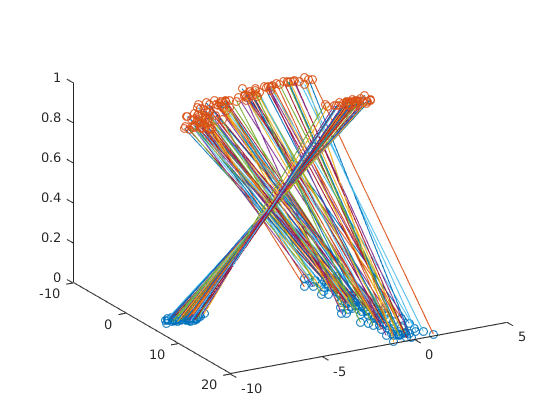
\includegraphics[width=15cm]{graphmatch.png}
  \caption{Example Graph matching. 150 nodes in both sets.}
  \label{fig:graphmatch}
\end{figure}

\section*{Next thing to do}

Obviously, there is a lot left to do. First, I want to update the algorithm to be able to handle a partial matching. The benefit of this algorithm is that the matrix $U$ gives a numerical value to the quality of matches between different points. We should be able to use this to decide what constitutes a ``good'' match, and which matches are ``bad''. In the final algorithm, we expect our input graphs to be sufficiently different, and we don't want to create any ``bad'' matches. Rather, we leave those points unmatched.

Second, we should be able to handle the case when $\abs{G_1}\neq\abs{G_2}$. Right now, the algorithm will run in this scenario, but the output doesn't seem optimal. See figure \ref{fig:graphmatch2}. In this example the set $X_1$ (blue) has 150 points, and $X_2$ (orange) has 90 points. When matching the line segments, it seems to prioritize points at the corners. I'm not sure why yet. I think those points are the most different from the points closer to the center of the line segments, which is why they are matched.

\begin{figure}
  \centering
  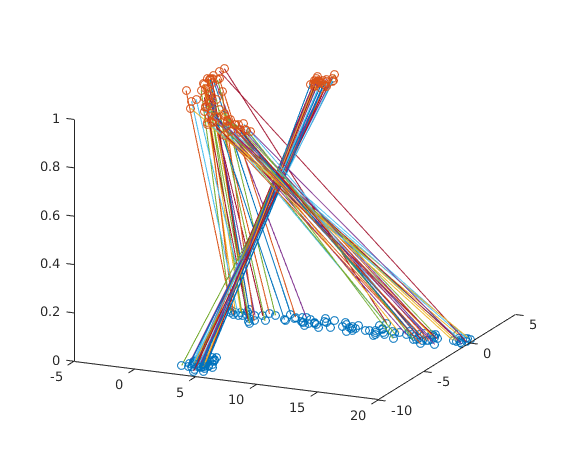
\includegraphics[width=15cm]{graphmatch2.png}
  \caption{150 nodes in blue set. 90 nodes in orange set.}
  \label{fig:graphmatch2}
\end{figure}

Third, maybe we should think about making this algorithm semisupervised. It's easy to enforce certain node-matchings by editing the matrix $U$ to give a high value to those matchings, but I don't think that fully uses the assumption that two nodes match. Somehow this should suggest more matchings with nearby nodes, but I'm not sure how to do that yet.

\end{document}